
\section{Objectif du site}
	\paragraph{}
		Le site doit permettre à des personnes de s’inscrire et se désinscrire de leur groupe à des session de sport. 
		
		
\section{Acteur}
	\paragraph{}
		\begin{itemize}
			\item Utilisateur : personne qui utilise le site et s'inscrivant à des session de sport
			\item Administrateur : personne administrant le site et ayant tout contrôle sur les sessions de sport organisé
		\end{itemize}
		

\section{User Stories}
	\subsection{Compatible Symfony-Twig et Symfony-Angular}
		\begin{center}
			\begin{tabularx}{\linewidth}{| Y | T{0.15\linewidth} |}
				\hline
				User Stories & Priority \\
				\hline
				En tant qu’utilisateur, je dois pouvoir me créer un compte sur le site & 2 \\
				\hline
				En tant qu’utilisateur, je dois pouvoir me connecter sur le site & 2 \\
				\hline
				En tant qu'utilisateur, je dois pouvoir sélectionner le mois et l'année pour afficher les sessions qui m'intéresse & 2 \\
				\hline
				En tant qu’utilisateur, je dois pouvoir m’inscrire à une session un certain jour & 1 \\
				\hline
				En tant qu’utilisateur, je dois pouvoir être inscrit automatiquement à une session & 1 \\
				\hline
				En tant qu’utilisateur, je dois pouvoir me désinscrire à une session & 1 \\
				\hline
				En tant qu’utilisateur, je dois pouvoir voir qui est inscrit pour chaque session & 2 \\
				\hline

			\end{tabularx}
		\end{center}
	
		\begin{center}
			\begin{tabularx}{\linewidth}{| Y | T{0.15\linewidth} |}
				\hline
				En tant qu’utilisateur, je veux pouvoir voir dynamiquement le nombre de séance qui reste dans mon abonnement & 2\\
				\hline
				En tant qu'utilisateur, je veux pouvoir modifier mon profile & 1\\
				\hline
				En tant qu'utilisateur, je veux pouvoir m'inscrire a une session uniquement si il me reste des abonnements a disposition. & 2\\
				\hline
				En tant qu’administrateur, je dois pouvoir annuler une session & 2 \\
				\hline
				En tant qu'administrateur, je dois pouvoir gérer les abonnement des utilisateurs & 2 \\
				\hline
			\end{tabularx}
		\end{center}
		
	\subsection{Compatible Symfony-Angular uniquement}
				\begin{center}
			\begin{tabularx}{\linewidth}{| Y | T{0.15\linewidth} |}
				\hline
				En tant qu'administrateur, je dois pouvoir créer un type de session & 2 \\
				\hline
				En tant qu'administrateur, je dois pouvoir générer les sessions pour un nombre d'année & 1 \\
				\hline
				En tant qu'administrateur, je veux pouvoir supprimer un utilisateur du système & 1\\
				\hline
				En tant qu'administrateur, je veux pouvoir gérer les types de sessions disponible pour l'inscription automatique & 2\\
				\hline
				En tant qu'administrateur, je veux pouvoir modifier un type de session & 1\\
				\hline
				En tant qu'administrateur, je veux pouvoir supprimer un type de session & 1\\
				\hline
			\end{tabularx}
		\end{center}

\vspace{\baselineskip}
\section{Contrainte non fonctionnelles}
	\paragraph{}
		\begin{itemize}
			\item Le site dois être user-friendly pour des personnes non adepte de la technologie. 
			\item Le site doit être responsive afin de pouvoir l'utiliser sur tout type de d'écran. 
		\end{itemize}

\newpage
\section{Mockup}
	\subsection{Login}
		\begin{figure}[!htbp]
       	 	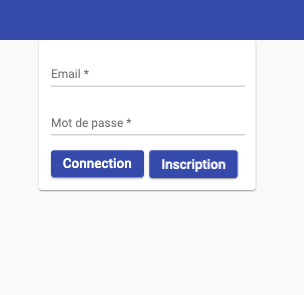
\includegraphics[width=0.5\linewidth, center]{Mockup/Login.png}
       	 	\caption{Page de connection}
       	\end{figure}
       	
    \vspace{\baselineskip}
	\subsection{Accueil}
		\begin{figure}[!htbp]
       	 	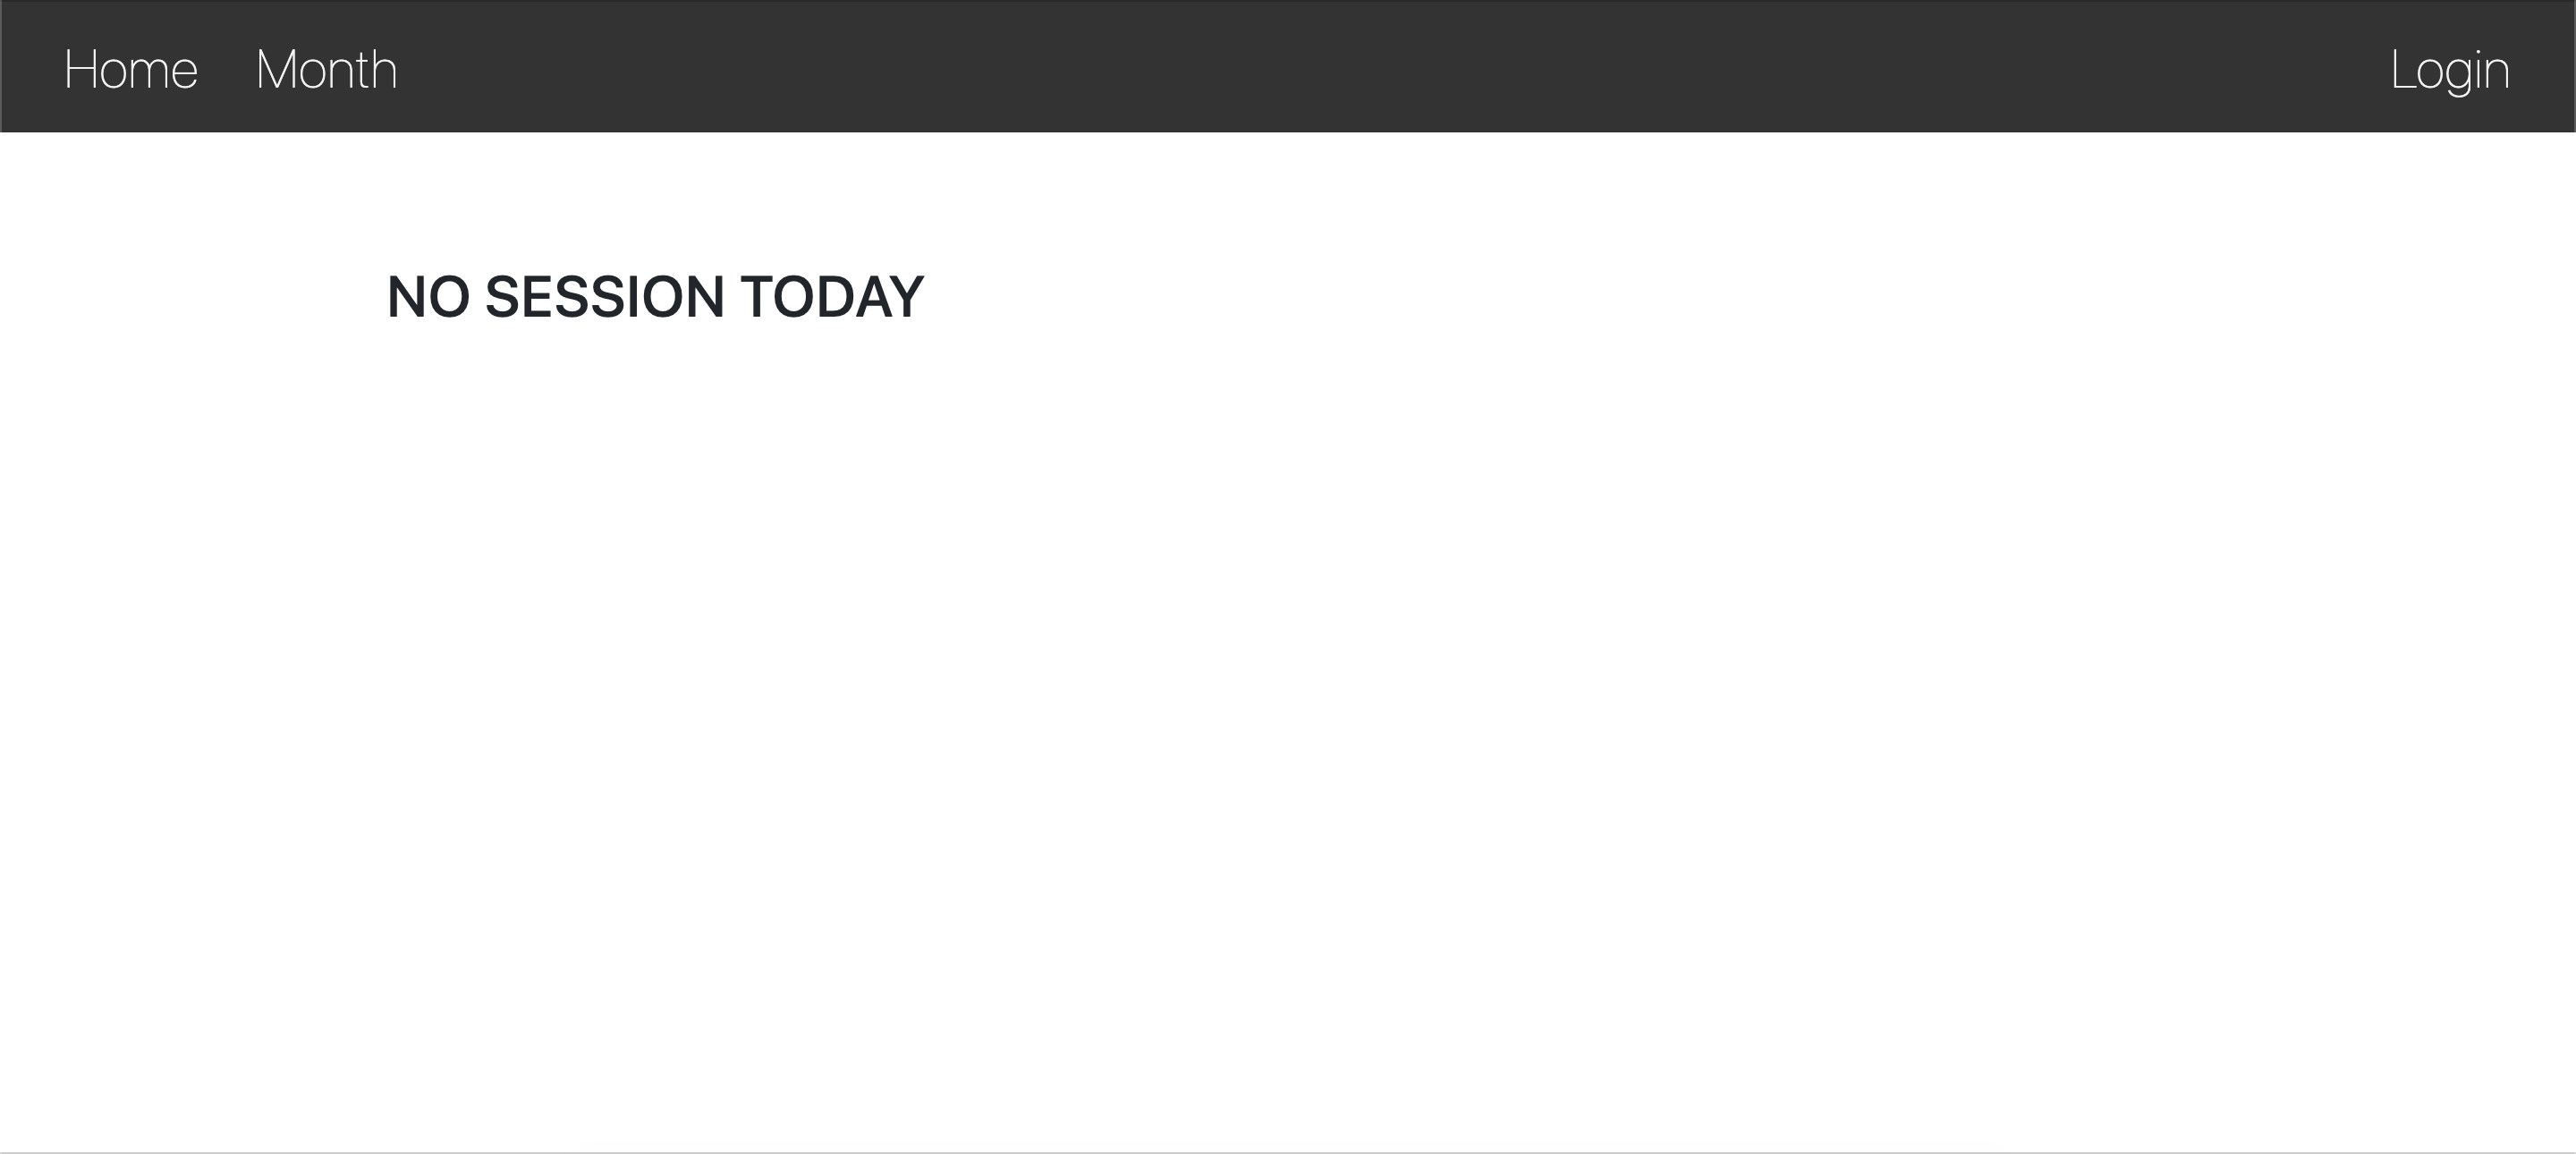
\includegraphics[width=0.8\linewidth, center]{Mockup/Accueil.png}
       	 	\caption{Page d'accueil}
       	\end{figure}
       	
       	
	\newpage
	\subsection{Inscription}
		\begin{figure}[!htbp]
       	 	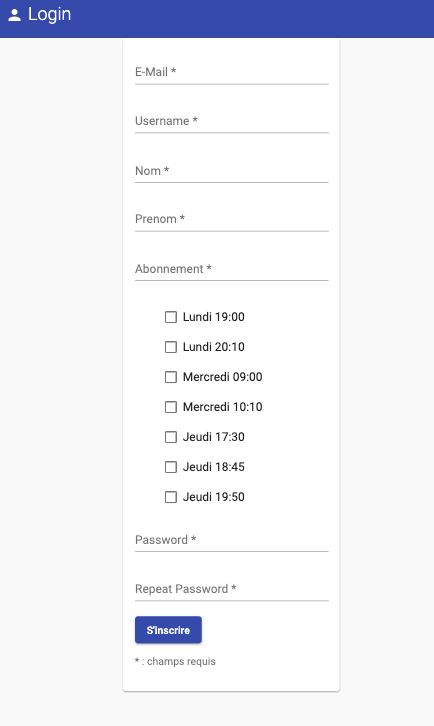
\includegraphics[width=0.5\linewidth, center]{Mockup/Inscription.png}
       	 	\caption{Page d'inscription au site}
       	\end{figure}
    
       
       
	\newpage
	\subsection{Month}
		\begin{figure}[h!]
       	 	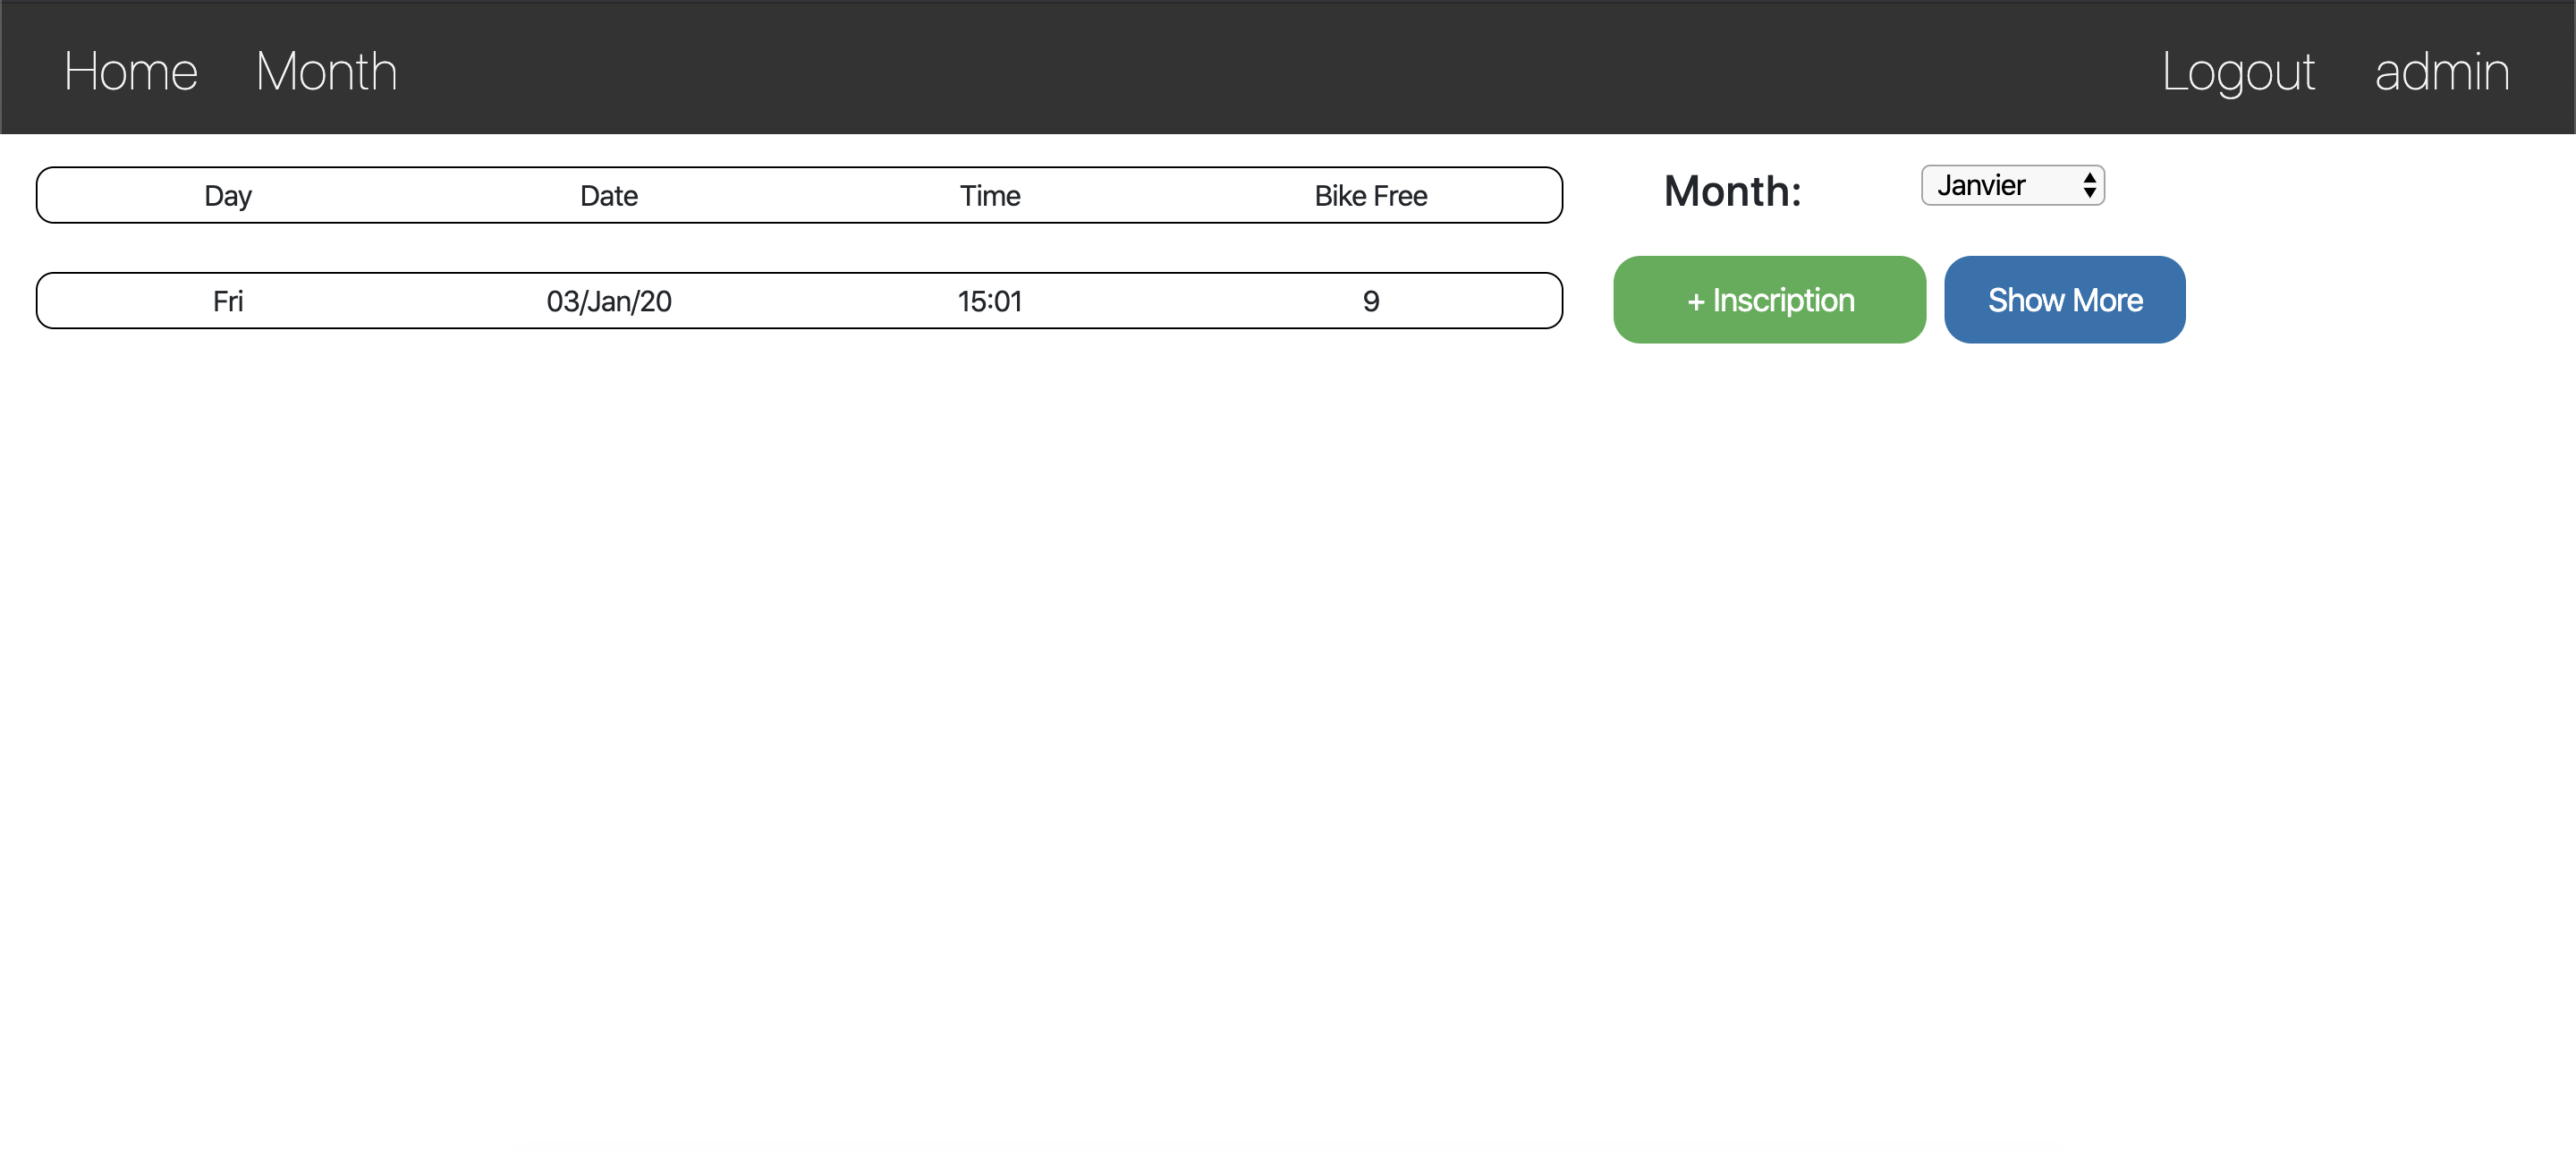
\includegraphics[width=0.8\linewidth, center]{Mockup/Month.png}
       	 	\caption{Page d'affichage des sessions du mois}
       	\end{figure}
       	

	\vspace{\baselineskip}	
	\subsection{Admin - Session}
		\begin{figure}[h!]
       	 	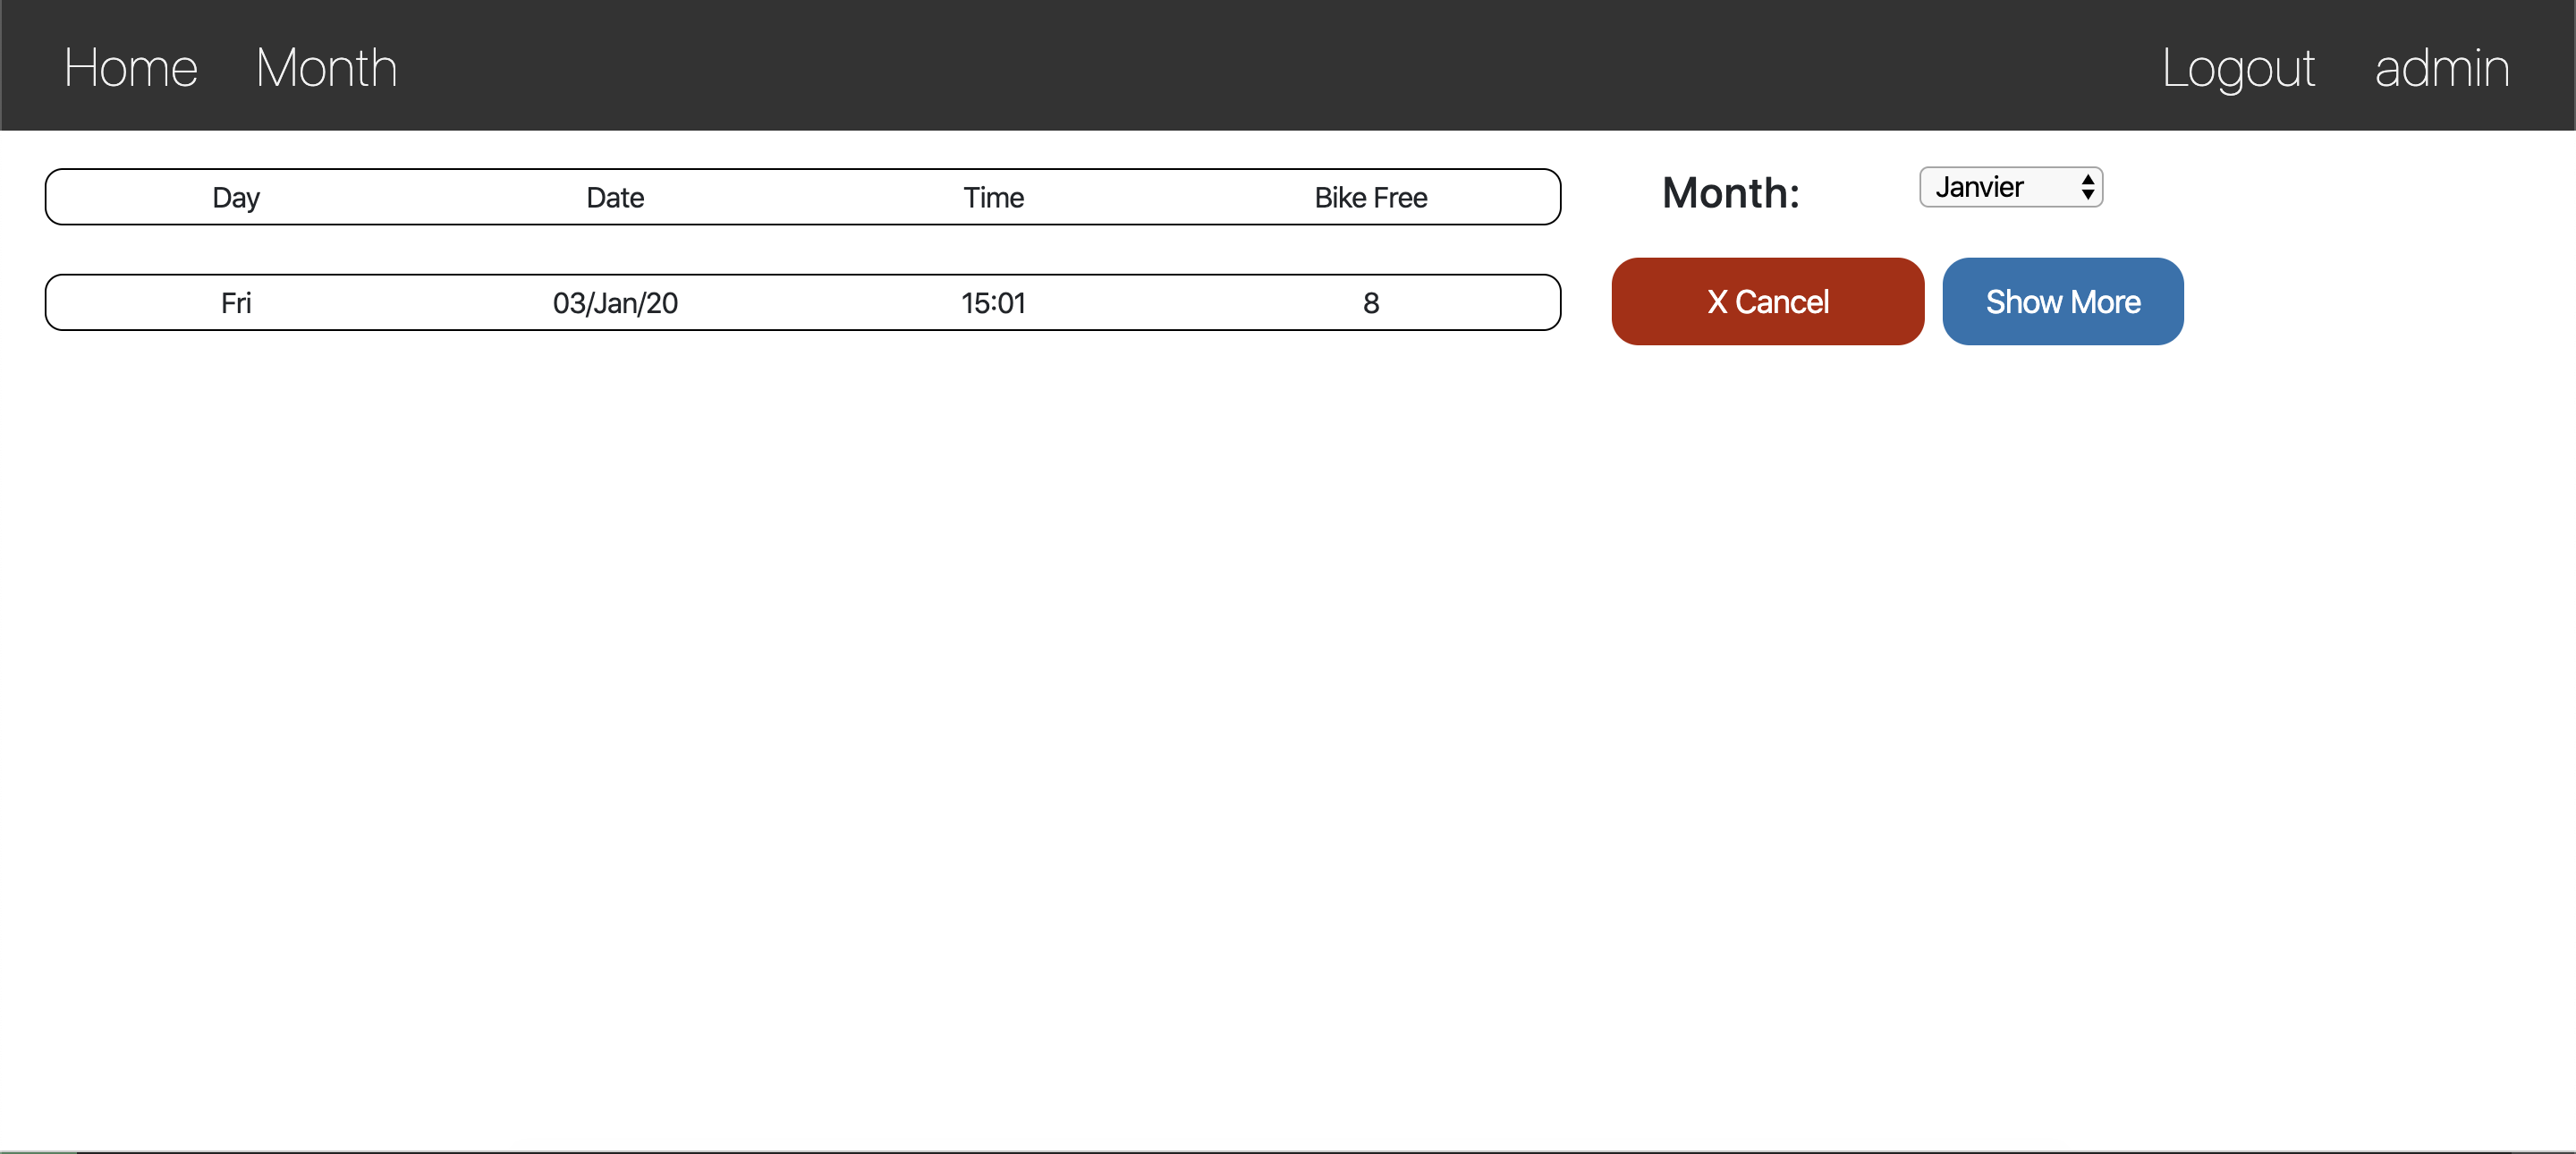
\includegraphics[width=0.8\linewidth, center]{Mockup/Admin-Session.png}
       	 	\caption{Page de gestion des sessions du mois pour l'administrateur}
       	\end{figure}
       	
	\newpage
	\subsection{Admin - NoHrefle session}
		\begin{figure}[h!]
       	 	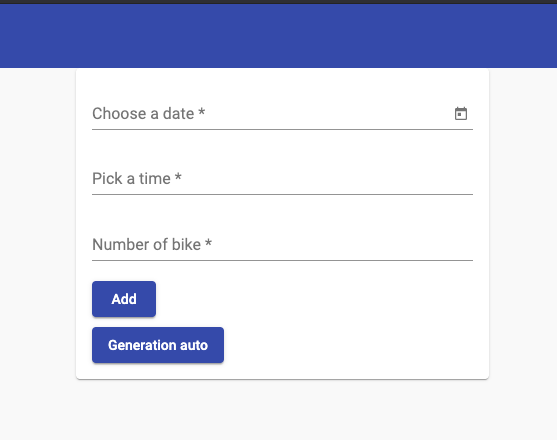
\includegraphics[width=0.8\linewidth, center]{Mockup/Admin-Nouvelle-Session.png}
       	 	\caption{Page de création d'une nouvelle session}
       	\end{figure}
       	
	\vspace{\baselineskip}
	\subsection{Admin - Abonnement}
		\begin{figure}[h!]
       	 	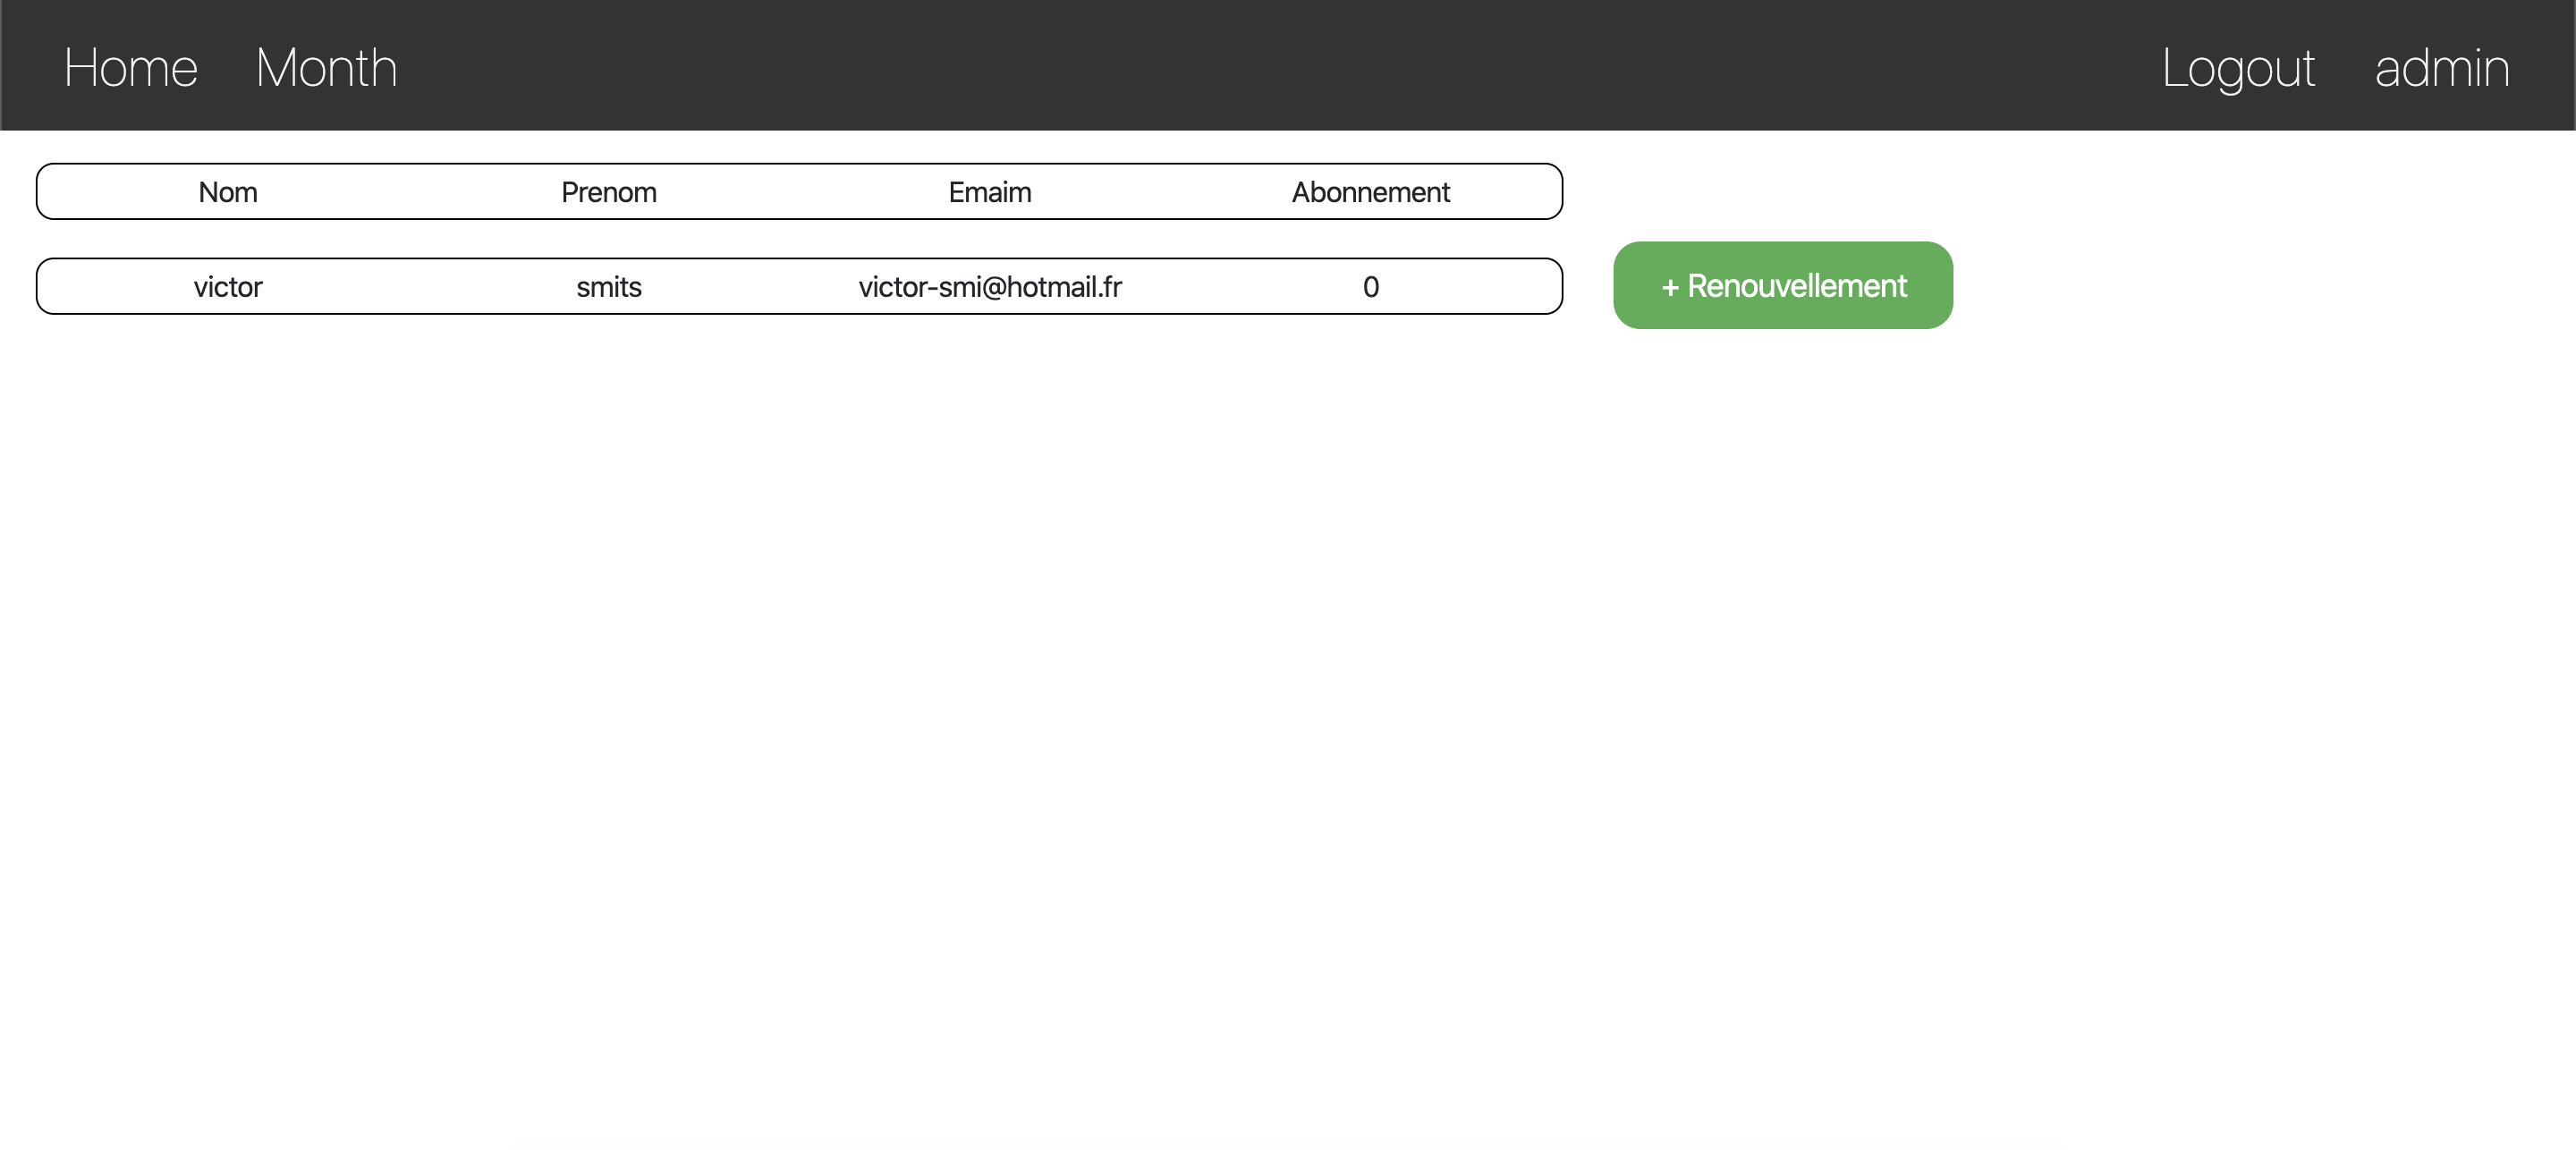
\includegraphics[width=0.8\linewidth, center]{Mockup/Admin-Abonnement.png}
       	 	\caption{Page de gestion des abonnements des utilisateurs}
       	\end{figure}
       	
	
	\newpage
	\subsection{Admin - Type Session}
		\begin{figure}[h!]
       	 	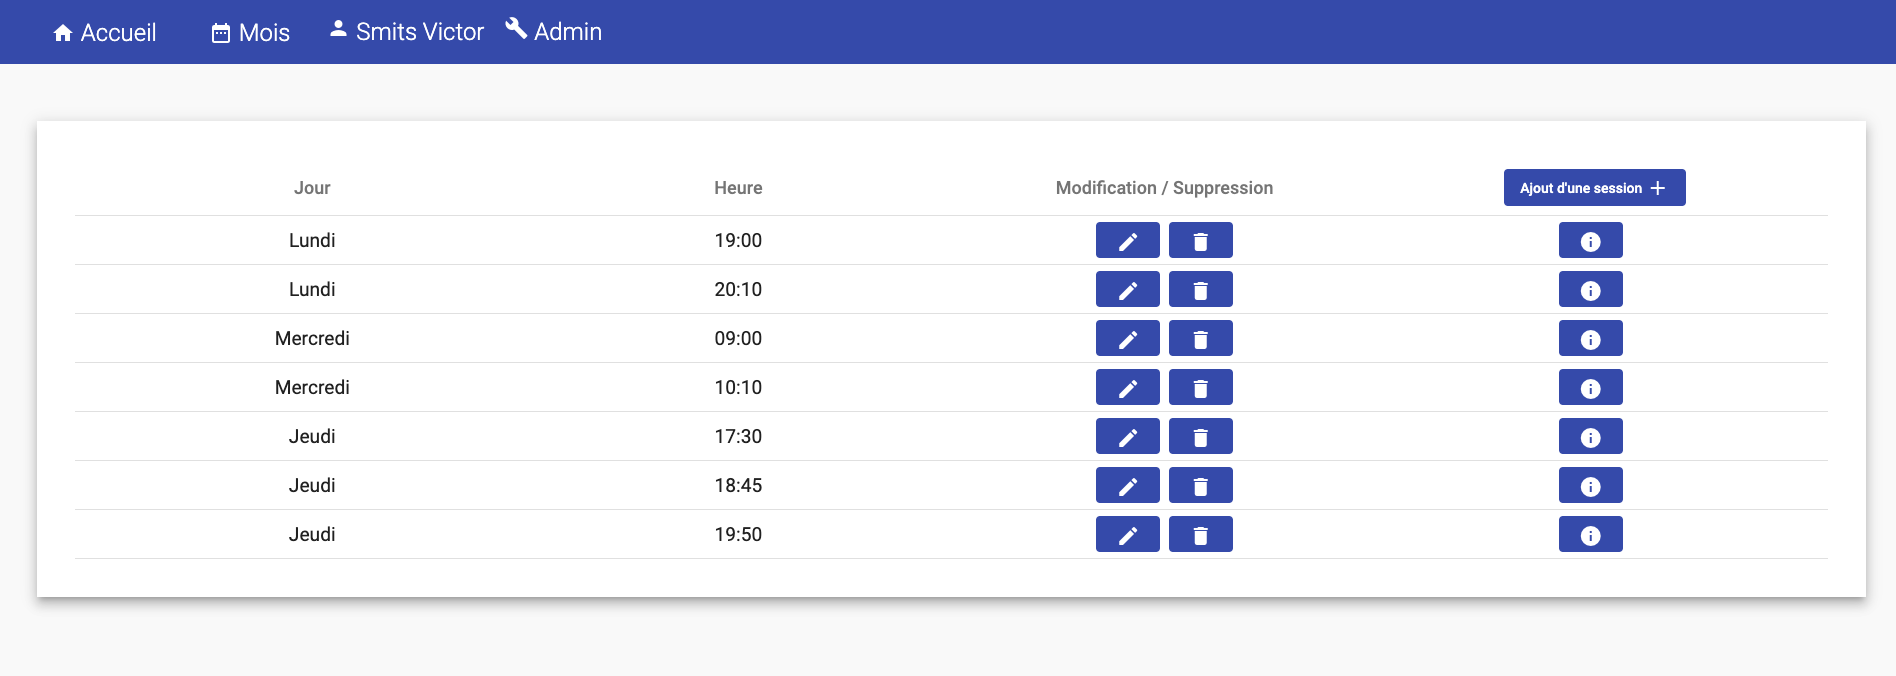
\includegraphics[width=0.8\linewidth, center]{Mockup/Admin-Type-Session.png}
       	 	\caption{Page de gestion des types de sessions}
       	\end{figure}

